\chapter{Vergleich der Cloud-Kosten}

Im folgenden Kapitel werden die monatlich anfallenden Cloud-Kosten \autocite{awsPricing} \autocite{gcpPricing} für die entwickelte Software am Standort Frankfurt verglichen. Die verwendeten Cloud-Dienste werden aus der Architektur extrahiert. Außerdem werden im Kapitel Anwendungsszenarien vorgestellt, um zu ermitteln, für welchen Fall welcher Dienst wirtschaftlicher ist.

\section{Kostenkategorien}

Dieser Unterabschnitt stellt zunächst die Kosten in unterschiedlichen Kategorien dar. Kosten, die nur für eine Cloud auftreten, werden in den sonstigen Kosten dargestellt.

\subsection{Hosting}

\begin{figure}%
    \centering
    \subfloat[\centering Gespeicherte Daten]{{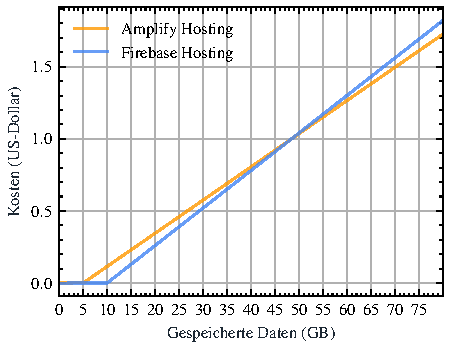
\includegraphics[width=6cm]{7_1_vergleich-cloud-kosten/hosting-stored-data.pdf} }}%
    \qquad
    \subfloat[\centering Übertragene Daten]{{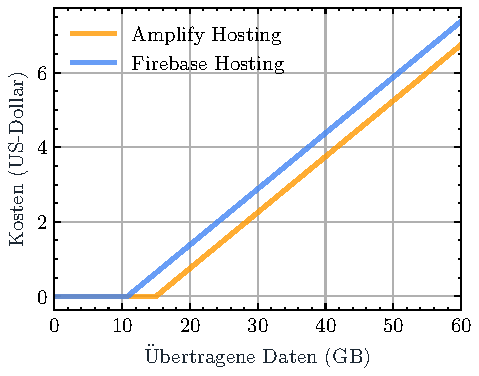
\includegraphics[width=6cm]{7_1_vergleich-cloud-kosten/hosting-transferred-data.pdf} }}%
    \caption{Kostenvergleich zwischen Amplify Hosting und Firebase Hosting}%
    \label{kostenvergleichHosting}%
\end{figure}

Beide Dienste benötigen den Hosting-Dienst, um das jeweilige Frontend zu speichern und auszuliefern. Dabei fallen Kosten für die Menge der gespeicherten Daten als auch für die Menge der übertragenen Daten an. \autoref{kostenvergleichHosting} stellt diesen Sachverhalt pro Kostenart dar.

\begin{description}
  \item[Gespeicherte Daten] Für das Amplify Hosting fallen \$ 0,023 pro GB an. Die ersten 5 GB sind kostenfrei. Für das Firebase Hosting fallen \$ 0,026 pro GB an. Die ersten 10 GB sind kostenfrei.
  \item[Übertragene Daten] Für beide Dienste fallen \$ 0,15 pro GB an. Lediglich das kostenlose Kontingent ist für das Amplify Hosting mit 15 GB gegenüber 10,8 GB für das Firebase Hosting etwas höher.
\end{description}

Für Projekte bis $\approx$ 48,33 GB sind die gespeicherten Daten in Firebase kostengünstiger. Für Projekte mit einem noch größeren Wert ist \ac{AWS} Amplify wirtschaftlicher. Bei Projekten mit bis zu 5 GB weist kein Tool einen Kostenvorteil aus, da beide noch kostenfrei sind. Die gespeicherten Daten hängen auch von der Anzahl der Builds ab. Demnach ist dieser Wert dann sinnvoll zu betrachten, wenn die Software hohe Entwicklungszyklen aufweist.

Die übertragenen Daten skalieren allerdings schneller als die gespeicherten Daten, da diese an die Anzahl der Nutzer gekoppelt sind, welche pro Aufruf ein Mal das Frontend herunterladen. Dabei ist kein wesentlicher Unterschied zwischen den beiden Diensten erkennbar, da das kostenlose Kontingent lediglich um 4,2 GB höher ist, was nur einen einmaligen Preisvorteil von maximal \$ 0,63 bringt.

Ein Vergleich der Build-Zeit findet an dieser Stelle nicht statt. \ac{AWS} Amplify selbst rechnet Build-Zeit mit \$ 0,01 pro Minute ab. Firebase Hosting bietet selbst keinen Build-Dienst als Gesamt-Deployment an. Daher muss dafür ein externer Dienst genutzt werden. Lediglich rechnet Google Cloud Functions die Dauer für das Deployment von einzelnen Funktionen ab.

Zusammenfassend lässt sich im Bereich Hosting kaum ein Kostenunterschied feststellen. Dies liegt daran, dass der  Proportionalitätsfaktor der übertragenen Daten bei beiden Diensten gleich ist.

\subsection{Serverless-Computing}

\begin{figure}
  \centering
  \subfloat[][\centering Ausführungszeit]{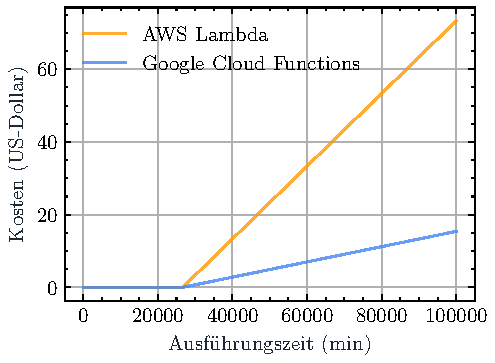
\includegraphics[width=.4\textwidth]{7_1_vergleich-cloud-kosten/functions-compute.pdf}}\quad
  \subfloat[][\centering Funktionsaufrufe]{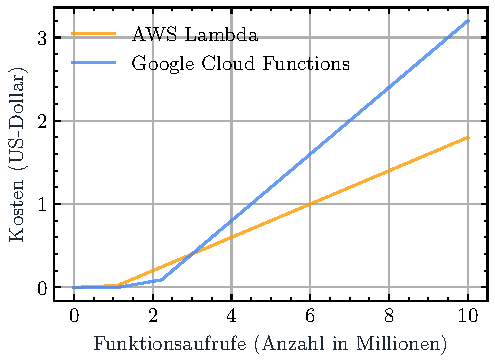
\includegraphics[width=.4\textwidth]{7_1_vergleich-cloud-kosten/functions-invocation.pdf}}\\
  \subfloat[][\centering Ausgehender Netzwerktransfer]{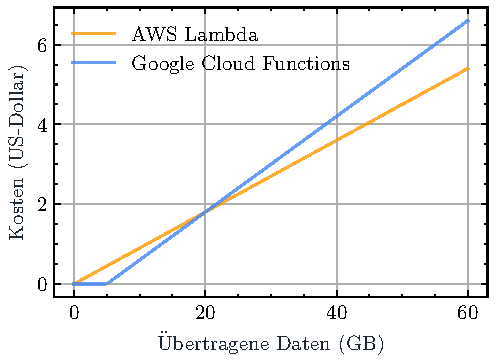
\includegraphics[width=.4\textwidth]{7_1_vergleich-cloud-kosten/functions-transfer.pdf}}\quad
  \caption{Kostenvergleich zwischen AWS Lambda und Google Cloud Functions}
  \label{kostenvergleichFunctions}
\end{figure}

Beide Dienste nutzen Serverless-Funktionen, um die Logik der Software abzubilden. Die Kosten unterteilen sich dabei in Ausführungs-, Aufruf- und ausgehende Netzwerkkosten. \autoref{kostenvergleichFunctions} stellt diesen Sachverhalt pro Kostenart dar. Die Angaben basieren auf 256 MB Arbeitsspeicher und der dazu gehörigen CPU mit einem x86-Prozessor. Außerdem werden für die Google Cloud die Tier-2 Preise genutzt, da diese für den Dienst in Frankfurt ausschlaggebend sind.

\begin{description}
  \item[Ausführungszeit] Für AWS Lambda fallen \$ 0,0000166667 pro GB-Sekunde an. Für Google Cloud Functions fallen \$ 0,0000035 pro GB-Sekunde an. Bei beiden Diensten sind die ersten 400000 GB-Sekunden kostenfrei.
  \item[Funktionsaufrufe] Für AWS Lambda fallen \$ 0,20 pro Millionen Aufrufen an. Die ersten 1 Millionen Aufrufe sind kostenfrei. Für Google Cloud Functions fallen \$ 0,40 pro Millionen Aufrufen an. Die ersten 2 Millionen Aufrufe sind kostenfrei.
  \item[Ausgehender Netzwerktransfer] Da in der entwickelten Software die Lambda-Funktionen von AppSync aufgerufen werden, gelten für den Netzwerktransfer die Preise dieses Services. Diese belaufen sich auf \$ 0,09 pro GB. Bei Google Cloud Functions sind es \$ 0,12 pro GB. Außerdem gibt es noch ein kostenloses Kontingent von 5 GB.
\end{description}

Auffällig ist, dass die Ausführung von Funktionen mit \ac{AWS} Lambda um mehr als ein 5-faches teurer ist als mit Google Cloud Functions. Allerdings ist der reine Vergleich irreführend, da die zu Grunde liegende Abrechnungsmethode beachtet werden muss. Während Lambda die Ausführungszeiten auf 1 ms rundet, wird bei Google Cloud Functions auf die nächsten 100 ms gerundet. Das bedeutet, dass eine Anfrage mit 10 ms auf 100 ms gerundet wird. Dabei würde dann das 10-fache der Nutzung bezahlt werden.

Auch bei den Funktionsaufrufen ist \ac{AWS} Lambda nach 3 Millionen Aufrufen nur halb so teuer wie Google Cloud Functions. Ein ähnliches Bild mit einem etwas geringeren Faktor ergibt sich bei dem Vergleich der Übertragungskosten.

Zusammenfassend gibt es für Software mit geringen Nutzerzahlen keinen wesentlichen Unterschied zwischen beiden Diensten. Jedoch ist mit steigender Nutzung \ac{AWS} Lambda wirtschaftlicher, da die Ausführungszeiten nicht nach oben gerundet werden und die Funktionsaufrufe deutlich günstiger sind.

\subsection{Storage}

\begin{figure}
  \centering
  \subfloat[][\centering Gespeicherte Daten]{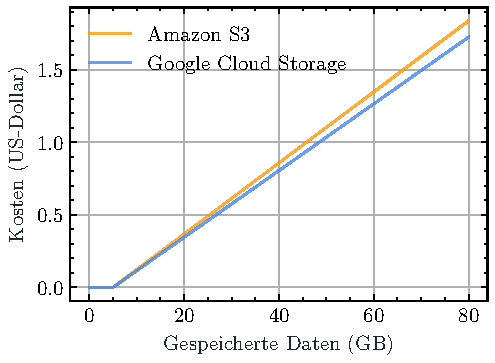
\includegraphics[width=.4\textwidth]{7_1_vergleich-cloud-kosten/storage-amount.pdf}}\quad
  \subfloat[][\centering Get-Anfragen]{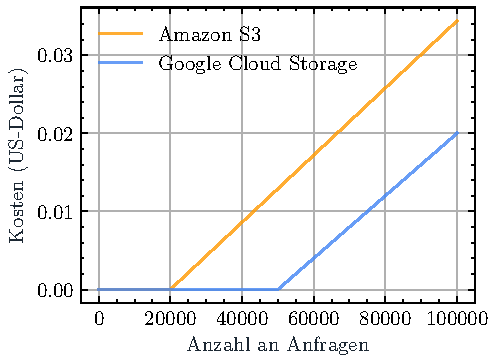
\includegraphics[width=.4\textwidth]{7_1_vergleich-cloud-kosten/storage-get.pdf}}\\
  \subfloat[][\centering Put/Post/List-Anfragen]{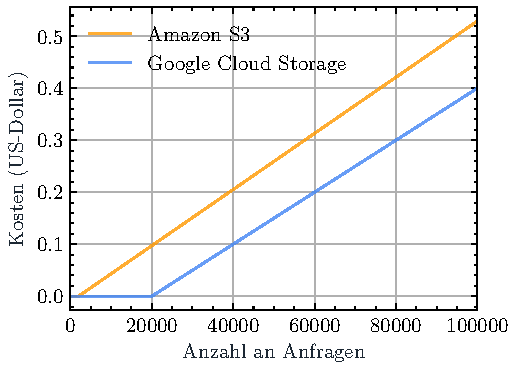
\includegraphics[width=.4\textwidth]{7_1_vergleich-cloud-kosten/storage-put.pdf}}\quad
  \subfloat[][\centering Ausgehender Netzwerktransfer]{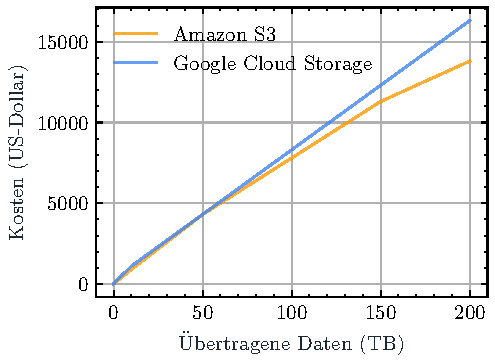
\includegraphics[width=.4\textwidth]{7_1_vergleich-cloud-kosten/storage-network.pdf}}
  \caption{Kostenvergleich zwischen Amazon S3 und Google Cloud Storage}
  \label{kostenvergleichStorage}
\end{figure}


AWS S3 mit Cloud Storage

S3

- Menge gespeicherter Daten
- Put, Post, List und Delete-Anfragen
- Get-Anfragen

Parameter
- S3 Standard Storage in GB
- PUT, COPY, POST, LIST Requests
- GET, SELECT Requests
- Inbound Data Transfer: Free
- Outbound Data Transfer: GB

Berechnung:
- S3 Standard Storage Costs: S3 Standard Storage in GB * 0.0245000000 USD
- S3 Standard PUT request costs: Number of PUT requests * 0.0000054 USD per request
- S3 Standard GET request costs: Number of GET requests * 0.00000043 USD per request
- Outbound Data Transfer:
    - 10240 GB x 0.09 USD per GB  (first 10TB)
    - 40960 GB x 0.085 USD per GB = 3481.60 USD (next 40TB)
    - 102400 GB x 0.07 USD per GB = 7168.00 USD (next 100TB)
    - 999846400 GB x 0.05 USD per GB = 49992320.00 USD (larger than 150TB)

Free tier: (für 12 Monate allerdings nur)
- 5 GB of Standard Storage
- 20,000 Get Requests
- 2,000 Put Requests

Ingress / Egress in beiden kostenlos

Cloud Storage (Standard Storage,
- Parameter
    - GB stored
    - Class A Operations: PUT, POST, LIST etc.
    - Class B Operations: GET
    - GB transferred
- Berechnung
    - Storage costs: $0.023 per GB / month
    - Class A = $0.05 per 10.000 Class A operations
    - Class B = $0.004 per 10.000 Class B operations
    - Transfer to Internet =  (Egress to Worldwide Destinations (excluding Asia & Australia) (per GB))
      - 0-1 TB $0.12
      - 1-10 TB	$0.11
      - 10+ TB $0.08

Free tier:
- 5GB storage
- 50k Class B
- 20K Class A
- 30 GB transfer


\subsection{Datenbank-Service}

DynamoDB mit Cloud Firestore

DynamoDB

Parameter:
- Data storage size in GB
- Average item size
- Writes
    - Standard writes vs Transactional writes: 100 / 0
    - Number of writes: 1000
- Reads
    - Eventually consistent vs Strongly vs Transactional: 100 / 0 / 0
    - Number of reads: 10 million per month
- On demand backup data storage

Free tier:
- 25 GB of Storage
- 25 provisioned Write Capacity Units (WCU)
- 25 provisioned Read Capacity Units (RCU)
- Enough to handle up to 200M requests per month.

Berechnung:
- Data storage costs: Data storage size * 0.306 USD
- Write costs: Number of writes * 0.000001525 USD
- Read costs: Number of reads x 1 strongly consistent portion x 1 read request units for strongly consistent reads x 25 read request units needed per item = 7,850,000,000.00 read request units for strongly consistent reads * 0.000000305 USD
- Backup storage costs: On demand backup data storage x 0.1224 USD



Cloud Firestore
- Parameter
    - GB stored
    - Document writes
    - Document reads
    - Document deletes
- Berechnung
    - Stored Data  = $0.117 per GB/ Month
    - Reads = $0.039/ 100.000 documents
    - Writes = $0.117 / 100.000 documents
    - Deletes = $0.013 / 100.000 documents
    - Transfer = ?

Free tier:
    Stored data	1 GiB
    Document reads	50,000 per day
    Document writes	20,000 per day
    Document deletes	20,000 per day
    Network egress	10 GiB per month


\subsection{Videokonvertierung}

\begin{figure}
  \centering
  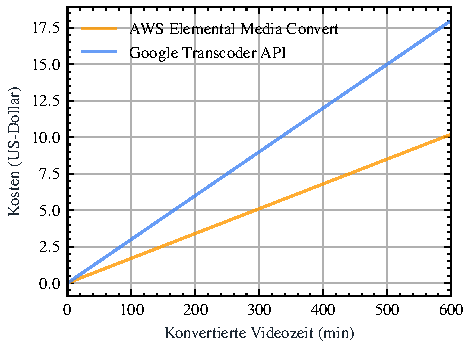
\includegraphics[width=0.75\columnwidth]{7_1_vergleich-cloud-kosten/transcoding.pdf}
  \caption{Kostenvergleich zwischen AWS Elemental Media Convert und Google Transcoder API}
  \label{KostenVideoTranscoding}
\end{figure}

Dieser Dienst wird genutzt, um das Wasserzeichen auf den hochgeladenen Videos zu platzieren. Die Werte beziehen sich auf die Konvertierung von Videos in HD-Qualität. Für \ac{AWS} Elemental Media Convert fallen \$ 0,017 pro Minute an. Für die Google Transcoder API fallen \$ 0,030 pro Minute an. \autoref{KostenVideoTranscoding} stellt diesen Zusammenhang dar. In diesem Bereich schneidet \ac{AWS} für jede Dauer besser ab.

\subsection{Sonstige}

Zu beachten ist zuletzt, dass einige Dienste für \ac{AWS} Amplify benötigt werden, die in Firebase nicht vorhanden sind oder in beiden Diensten nicht abgerechnet werden.
\begin{description}
\item[User Management] Da die erweiterten Sicherheitsfunktionalitäten von \ac{AWS} Cognito nicht genutzt werden, ist dieser kostenfrei. Auch seitens Firebase gibt es für das User-Management keine extra Kosten für die Standardfunktionalität.
\item[Benachrichtigung von Diensten] Amazon EventBridge wird verwendet, um \ac{AWS} Lambda darüber zu benachrichtigen, dass ein Video erfolgreich konvertiert wurde. Der Dienst kostet pro 1 Millionen Custom Events \$ 1,00. In Firebase ist dafür kein zusätzlicher Dienst nötig.
\item[GraphQL] Aufgrund von Unterschieden in der Architektur nutzt \ac{AWS} Amplify mit AWS AppSync einen GraphQL-Server, während Firebase ohne einen solchen auskommt, da Funktionen direkt aus dem Frontend aufgerufen werden können. Bei \ac{AWS} entstehen dadurch Nutzungskosten von \$ 4,00 für 1 Millionen Queries oder Mutations. Außerdem entstehen Datentransferkosten. Diese sind allerdings schon durch die Netzwerkkosten aus \ac{AWS} Lambda abgedeckt.
\end{description}

\subsection{Zusammenfassung}

zusammenfassung aller dienste und wo welcher dienst günstiger ist

\section{Preisbeispiele}

- Szenarien 1 2 3 ggf. auch nur eins

TODO: Nutzungsprofile für die Anwendung definieren, damit der vergleich einfacher ist